\chapter{Electric Fields in Matter}

\section{Polarization}\label{polarization}

\subsection{Dielectrics}

Most everyday objects belong to one of two large classes: \vocab{conductors} and \vocab{insulators} (or \vocab{dielectrics}).

\begin{definition}
In an \vocab{insulator}, all charges are attached to specific atoms or molecules. They're on a tight leash, and all they an do is move a little \textit{within} the atom or molecule.
\end{definition}

This is in contrast to conductors, where there is an ``unlimited" supply of charges that are free to move around throughout the material, without being attached to particular atoms or molecules.

The microscopic displacements within a dielectric material is not as dramatic as the rearrangement of charge in a conductor, but their effects account for the characteristic behavior of dielectric materials. External electric fields can distort the charge distribution of a dielectric atom or molecule in \textit{two} ways: \textit{stretching} and \textit{rotating}.

\subsection{Induced Dipoles}\label{induceddipoles}

What happens when a neutral atom is placed in an electric field $\vec{E}$? 

An initial guess is that nothing should happen: the atom is not charged, so the field has no effect on it. However, this is incorrect. Even though the atom \textit{as a whole} is electrically neutral, there is still a positively charged core (the nucleus) and negatively charged electron cloud surrounding it. These two regions are pushed and pulled by the field.

If the field is large enough, then this could be enough to pull the atom apart completely, ``ionizing" it into a conudctor. With less extreme fields, however, an equilibrium is established as the positive and negative charges attract one another, holding the atom together. 

This leaves the atom \vocab{polarized}, with plus charge shifted slightly in the direction of the field and the minus charge the other way. The atom now has a tiny dipole moment $\vec{p}$, which points in the \textit{same direction} as $\vec{E}$. Typically, these are roughly proportional
\[\vec{p}=\alpha\vec{E},\]
where the constant of proportionality is called the \vocab{atomic polarizability}.

\begin{example}\label{primatompolar}
A primitive model for an atom consists of a point nucleus $(+q)$ surrounded by a uniformly charged spherical cloud $(-q)$ of radius $a$. Calculate the atomic polarizability of such an atom.
\end{example}

\begin{proof}
Suppose the $+q$ nucleus is shifted a distance of $d$ in the direction of the electric field $\vec{E}$. Then, the field due to the spherical cloud pulling it back should be equal to $E$. Hence,
\[\frac{1}{4\pi\varepsilon_0}\cdot \frac{q\cdot d^3/a^3}{d^2}=\frac{qd}{4\pi\varepsilon_0 a^3},\]
so $p=4\pi\varepsilon_0 a^3\cdot E$. Hence,
\[\alpha=4\pi\varepsilon_0a^3=3\varepsilon_0 v,\]
where $v$ is the volume of the atom.
\end{proof}

\begin{remark}
Though this model is quite crude, the result isn't actually that bad---it's accurate within a factor of four or so for many simple atoms.
\end{remark}

Molecules are not as simple as atoms, since frequently they can polarize more easily in some directions than in others. For example, carbon dioxide has a polarizability of $4.5\times 10^{-40} \text{ C}^2\cdot\text{m}/\text{N}$ when a field is applied along the axis of the molecules, but only $2\times 10^{-40}$ for fields perpendicular to the axis. Therefore, if the field is at some angle to the axis, we resolve it into parallel and perpendicular components:
\[\vec{p}=\alpha_\perp\vec{E}_\perp + \alpha_\parallel \vec{E}_\parallel.\]
In these cases, the induced dipole moment may \textit{not} be in the same direction as $\vec{E}$.

For more general molecules (i.e. a completely asymmetrical molecule), we replace the equation with the most general linear relation between $\vec{E}$ and $\vec{p}$:
\[\begin{bmatrix}
p_x \\ p_y \\ p_z
\end{bmatrix}=\begin{bmatrix}
\alpha_{xx} & \alpha_{xy} & \alpha_{xz}\\
\alpha_{yx} & \alpha_{yy} & \alpha_{yz}\\
\alpha_{zx} & \alpha_{zy} & \alpha_{zz}
\end{bmatrix}\cdot\begin{bmatrix}
E_x \\ E_y \\ E_z
\end{bmatrix}.\]
The set of nine constants $\alpha_{ij}$ make up the \vocab{polarizability tensor} for the molecule. These values depend on the orientation of the coordinate axes that we choose, but note that we can always choose ``principal" axes so that the off-diagonal terms vanish (the matrix is diagonalizable).

\subsection{Alignment of Polar Molecules}

The neutral atom discussed in Example \ref{primatompolar} had no dipole moment to start with: $\vec{p}$ was induced by the external electric field $\vec{E}$. However, some molecules have built-in, permanent dipole moments. For example, in a water molecule, the electrons tend to cluster around the oxygen atom, and since it is bent at $105^\circ$, there is a negative charge built up at the vertex and a positive charge on the opposite side. The dipole moment thus generated is unusually large: $6.1\times 10^{-30}\text{ C}\cdot\text{m}$.

What happens when such \vocab{polar molecules} are placed in an electric field? Well, the \textit{force} on the positive end exactly cancels out the force on the negative end, but a torque is induced:
\begin{align*}
\vec{N}&=(\vec{r}_+\times \vec{F}_+)+(\vec{r}_-\times \vec{F}_-)\\
&=\left[(\vec{d}/2)\times (q\vec{E})\right]+\left[(-\vec{d}/2)\times (-q\vec{E})\right]=q\vec{d}\times \vec{E}.
\end{align*}
Thus a dipole $\vec{p}=q\vec{d}$ in a uniform field $\vec{E}$ experiences a torque
\[\vec{N}=\vec{p}\times\vec{E}.\]
Note that $\vec{N}$ is in a direction which tries to line $\vec{p}$ up with $\vec{E}$. Therefore, a polar molecule that is free to rotate will swing around until it points in the direction of the applied field.

If the field is \textit{nonuniform}, then there will be a net \textit{force} on the dipole, in addition to the torque. Normally this is not much of an issue, since $\vec{E}$ would have to change very abruptly in teh space of one molecule. Nonetheless, we have
\[\vec{F}=\vec{F}_++\vec{F}_-=q(\vec{E}_+-\vec{E}_-)=q(\Delta \vec{E}).\]
If the dipole is short, we can approximate the small change in $E_x$ along the direction $\vec{d}$ by
\[\Delta E_x=(\nabla E_x)\cdot \vec{d}.\]
This gives
\[\Delta\vec{E}=(\vec{d}\cdot \nabla)\vec{E},\]
so
\[\vec{F}=(\vec{p}\cdot \nabla)\vec{E}.\]

\subsection{Polarization}

So, what happens to a piece of dielectric material when it is placed in an electric field? From our discussion in the previous sections:\footnote{The actual process is not quite as clear-cut as these two bullets would suggest: polar molecules also experience some polarization by displacement (though generally rotation is much easier so that's the dominant effect), and some materials retain their polarization after the field is removed.}
\begin{itemize}
    \item If the substance consists of neutral atoms (or nonpolar molecules), the field will induce a tiny dipole moment pointing in the same direction as the field.
    \item If the substance consists of polar molecules, each permanent dipole will experience a torque, tending it to line up along the direction of the field (though random thermal motions will compete with this process).
\end{itemize}
The net result, either way, is that we end up with a lot of little dipoles pointing along the direction of the field, making the material \vocab{polarized}. A measure of this effect is the \vocab{polarization} $\vec{P}$, defined as the dipole moment per unit volume.

In the next section, we will study the field that a chunk of polarized material \textit{itself} produces. After that, we will put together the original field that caused $\vec{P}$ and the new field due to $\vec{P}$.

\section{The Field of a Polarized Object}\label{fieldofpolarized}

\subsection{Bound Charges}

The main question of this section is to find the field produced by an object with polarization $\vec{P}$ (i.e. dipole moment per unit volume) given.

We work with potentials. For a single dipole $\vec{p}$, recall that
\[V(\vec{r})=\frac{1}{4\pi\varepsilon_0}\frac{\vec{p}\cdot\hat{\scr}}{\scr^2},\]
where $\scr$ is the separation vector from the dipole to the point at which we are evaluating the potential, $\vec{r}$. Since we have a dipole moment $\vec{p}=\vec{P}d\tau'$ for each volume element $d\tau'$, we simply integrate for the total potential:
\[V(\vec{r})=\frac{1}{4\pi\varepsilon_0}\iiint_{\mathcal{V}}\frac{\vec{P}(\vec{r'})}{\scr^2}d\tau'.\]
In principle, we are done, but we can rearrange this into a more enlightening form by noting that
\[\nabla'\left(\frac{1}{\scr}\right)=\frac{\hat{\scr}}{\scr^2},\]
where the differentiation in $\nabla'$ is with respect to the \textit{source} coordinates in $\vec{r;}$. Hence, applying integration by parts gives
\begin{align*}
    V&=\frac{1}{4\pi\varepsilon_0}\iiint_{\mathcal{V}}\vec{P}\cdot \nabla'\left(\frac{1}{\scr}\right)d\tau'\\
    &=\frac{1}{4\pi\varepsilon_0}\left[\iiint_{\mathcal{V}}\nabla'\cdot\left(\frac{\vec{P}}{\scr}\right)d\tau'-\iiint_{\mathcal{V}}\frac{1}{\scr}(\nabla'\cdot \vec{P})d\tau'\right]\\
    &=\frac{1}{4\pi\varepsilon_0}\oiint_{\partial\mathcal{V}}\frac{\vec{P}}{\scr}\cdot d\vec{a'}-\frac{1}{4\pi\varepsilon_0}\iiint_{\mathcal{V}}\frac{1}{\scr}(\nabla'\cdot \vec{P})d\tau'.
\end{align*}
We define two quantities:
\begin{definition}
In a polarized dielectric, we define two \vocab{bound charges} $\sigma_b$ and $\rho_b$. The surface bound charge is given by
\[\sigma_b:=\vec{P}\cdot \hat{n},\]
while the volume bound charge is given by
\[\rho_b:=-\nabla\cdot\vec{P}.\]
\end{definition}

With these definitions, we simply have
\[V(\vec{r})=\frac{1}{4\pi\varepsilon_0}\oiint_{\partial\mathcal{V}}\frac{\sigma_b}{\scr}da'+\frac{1}{4\pi\varepsilon_0}\iiint_{\mathcal{V}}\frac{\rho_b}{\scr}d\tau'.\]
The first term here is simply the potential generated by a surface charge density $\sigma_b$, while the second term here is simply the potential generated by a volume charge density $\rho_b$.

\begin{remark}\label{boundchargeintuition}
In the next subsection, we will see how these bound charges correspond to actual accumulations of charge within the dielectric. I'd encourage you to think about why this would be true! (Think of a bunch of little electric dipoles.)
\end{remark}

Therefore, instead of integrating the contributions of all the individual infinitesimal dipoles, we could first calculate the bound charges, and then calculate the fields \textit{they} produce, using any standard techniques we use for surface or volume charges (e.g. Gauss's Law).

\begin{example}
Find the electric field produced by a uniformly polarized sphere of radius $R$.
\end{example}

\begin{proof}
Let the direction of polarization point along the positive $z$-axis. Since $\vec{P}$ is uniform, it is simple to compute the bound charges:
\[\sigma_b=\vec{P}\cdot \hat{n}=P\cos\theta \qquad \text{and} \qquad \rho_b=-\nabla\cdot\vec{P}=0.\]
Recall that in Example \ref{chargespherepotential} and the following remark, we computed the potential generated by such a spherical charge distribution to be
\[V(r,\theta)=\begin{dcases}
\frac{P}{3\varepsilon_0}r\cos\theta & \text{if } r\le R,\\
\frac{P}{3\varepsilon_0}r\left(\frac{R}{r}\right)^3\cos\theta & \text{if } r\ge R.
\end{dcases}\]
For the electric field inside the sphere, simply note that $r\cos\theta=z$, so the field inside is actually \textit{uniform}!
\[\vec{E}=-\nabla V=-\frac{P}{3\varepsilon_0}\hat{z}=-\frac{1}{3\varepsilon_0}\vec{P}\qquad (r<R).\]
Meanwhile, outside the sphere, the potential is actually just identical to a perfect dipole at the origin with dipole moment $\vec{p}=\frac{4}{3}\pi R^3\vec{P}$ (not very surprising, as this is the total dipole moment):
\[V=\frac{1}{4\pi\varepsilon_0}\frac{\vec{p}\cdot\hat{r}}{r^2}\qquad (r\ge R).\]
Here's a picture:
\begin{center}
    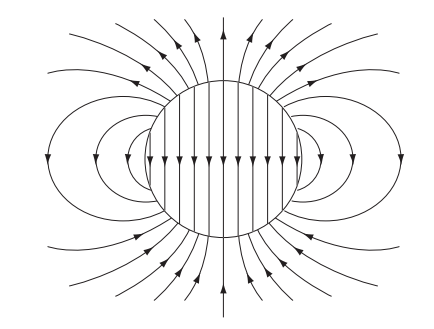
\includegraphics[width=8cm]{Electrodynamics/images/fig4.10.PNG}
\end{center}
\end{proof}

\subsection{Physical Interpretation of Bound Charges}

In the last section, we showed that instead of integrating over each of the tiny dipoles in a polarized dielectric material, we could simply compute some bound charge densities $\sigma_b$ and $\rho_b$ using $\vec{P}$ and then determine the field of these charges.

While we found the formulas $\sigma_b=P\cdot \hat{n}$ and $\rho_b=-\nabla\cdot \vec{P}$ using a mathematical trick, it turns out that there is a physical interpretation for these bound charges: they actually represent \textit{real, genuine accumulations of charge} within the dielectric material, as hinted at in Remark \ref{boundchargeintuition}.

The basic idea is very similar to the intuitive proof of Stokes' theorem: if we each little dielectric as a small $+$ next to a small $-$, we notice that these can often cancel each other. For a first example, imagine a string of dipoles lined up (with constant polarization), as shown below. The $+$ charge of one dipole will cancel with the $-$ charge of the next dipole, resulting in the only remaining charges being the bound $-$ on one end and bound $+$ on the other.

\begin{center}
    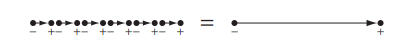
\includegraphics[width=8cm]{Electrodynamics/images/fig4.11.PNG}
\end{center}

To calculate the actual amount charge, consider a tube of dielectric parallel to $\vec{P}$. Consider the chunk of dielectric with dipole moment $P(Ad)$ shown on the left; it is equivalent to a dipole with charge $q=PA$. Hence the bound charge that piles up at the right end of the tube is $q=PA$.

Note that if the ends of the tube are indeed perpendicular to $\vec{P}$, then the surface charge density is simply $\sigma_b=P$, but if sliced diagonally, the \textit{total} charge should remain the same, but the new area is $A_{\text{end}}=\frac{A}{\cos\theta}$< so the surface charge density is instead $\vec{P}\cdot \hat{n}$ (which matches for the case where $\hat{n}$ is parallel to $\vec{P}$, anyway). 

\begin{center}
    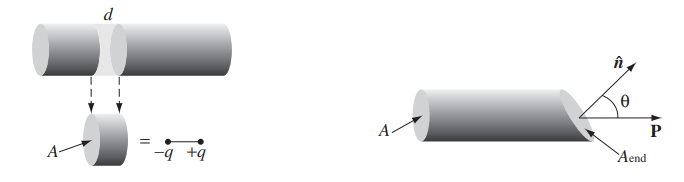
\includegraphics[width=10cm]{Electrodynamics/images/fig4.12-13.PNG}
\end{center}

Thus, we conclude that the effect of polarization of a dielectric is a bound charge of $\sigma_b=\vec{P}\cdot\hat{n}$ over the surface of the material.

So, where does the volume bound charge $\rho_b$ come from? Well, so far, we've only considered situations where $\vec{P}$ is uniform. If it's not, then we expect some accumulation of charge within the material. For example, if we have a strong area of polarization pointing into a weaker area of polarization, we expect an accumulation of positive charge within the material at that location. As for another example, consider the figure below:

\begin{center}
    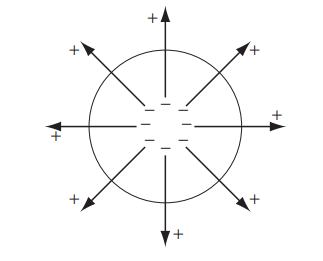
\includegraphics[width=8cm]{Electrodynamics/images/fig4.14.PNG}
\end{center}

This immediately suggests that a diverging $\vec{P}$ results in an accumulation of negative charge. Indeed, if we consider the net bound charge in a particular volume $\mathcal{V}$, it should be equal and opposite to the amount of charge that is pushed out of the surface (which, as we've already reasoned, should be $\vec{P}\cdot\hat{n}$):
\[\iiint_{\mathcal{V}}\rho_bd\tau=-\oiint_{\partial\mathcal{V}}\vec{P}\cdot d\vec{a}=-\iiint_{\mathcal{V}}(\nabla\cdot \vec{P})d\tau.\]
Since this is true for \textit{any} volume, we must have $\rho_b=-\nabla\cdot \vec{P}$.

\begin{remark}
We can also interpret a uniformly polarized sphere as simply \textit{two} spheres of charge; a positive sphere and a negative sphere, superimposed. When the sphere is polarized, all the plus charges move slightly upwards and all the minus charges move slightly downwards (assuming polarization in the $\hat{z}$ direction). The leftover caps of charges is precisely the bound surface charge $\sigma_b$, while there is no charge accumulation $\rho_b$ inside since $\vec{P}$ is uniform.

For the field inside, you can easily compute it as uniform, and you'll get the same result of 
\[\vec{E}=-\frac{1}{3\varepsilon_0}\vec{P},\]
as before. For the field outside the sphere, we can simply imagine the charge on each sphere as concentrated in its center, so we get that the field outside is the same as a perfect dipole at the center (since the shift $\vec{d}$ between the centers of the negative and positive spheres is miniscule, at the scale of one atomic radius).
\end{remark}

% \subsection{The Field Inside a Dielectric (Optional)}

% In this section, we have mostly neglected any difference between physical and perfect dipoles; indeed, we started with pure dipoles making up the material. Yet, an actual polarized material consists of physical dipoles, even if they are small.

% Outside the material, this is fine. We are far away from these tiny dipoles, so the dipole potential is essentially correct. Yet what about \textit{inside} the material? We can hardly assume that that we are far away from the dipoles!

% Well, inside \textit{any} material, the actual \vocab{microscopic} electric field \textit{must} be fantastically complicated. After all, it must be massive in magnitude, say, really close to an electron, while just a short distance away it could be really small or in a completely different direction. Therefore, just as how we consider water to be a continuous fluid rather than truly being a bunch of microscopic particles, we only concentrate on the \vocab{macroscopic} electric field within a dielectric.

% To do so, we need to pick some characteristic radius (say, 1000 times the diameter of an atom) and average the electric field over it, enough to smooth over the microscopic bumps but also pick up on any large-scale variations (much like as we do for fluid mechanics when calculating pressure).

\section{The Electric Displacement}\label{electricdisplacement}

\subsection{Gauss's Law in the Presence of Dielectrics}

In the last section we found that the net effect of polarization is to produce accumulations of bound charge, $\rho_b=-\nabla\cdot \vec{P}$ inside the dielectric and $\sigma_b=\vec{P}\cdot\hat{n}$ on its surface. The electric field due to the polarized object is then just the field of this bound charge.

Now we will put everything together: this field generated by the bound charge \textit{plus} the field generated due to everything \textit{else}.

\begin{definition}
Any charge that is \textit{not} a result of polarization (i.e. not bound charge) we call \vocab{free charge} $\rho_f$.
\end{definition}

The free charge might consist of electrons on a conductor or ions embedded in the dielectric material. Therefore, within the dielectric, we have
\[\rho=\rho_b+\rho_f,\]
so Gauss's law reads
\[\varepsilon_0\nabla\cdot \vec{E}=\rho=\rho_b+\rho_f=-\nabla\cdot \vec{P}+\rho_f.\]
Rearranging gives 
\[\nabla\cdot(\varepsilon_0\vec{E}+\vec{P})=\rho_f,\]
which motivates the following definition:
\begin{definition}
We call the quantity 
\[\vec{D}:=\varepsilon_0\vec{E}+\vec{P}\]
the \vocab{electric displacement}.
\end{definition}

\begin{theorem}[Gauss's Law for Dielectrics]
We have
\[\nabla\cdot \vec{D}=\rho_f,\]
or, in integral form,
\[\oiint \vec{D}\cdot d\vec{a}=Q_{f,\text{enc}},\]
where $Q_{f,\text{enc}}$ is the total amount of free charge enclosed in the volume.
\end{theorem}

This equation is particularly useful since the free charge is the stuff we can control; bound charge comes along when we place dielectrics in the area, where the mechanisms discussed at the start of the chapter induce \textit{some} polarization, causing some bound charge. Therefore, in a problem, we know $\rho_f$, but not (at least, initially) $\rho_b$. If the standard symmetries are present (e.g. spherical, cylindrical), we can use Gauss's law to immediately calculate $\vec{D}$.

\begin{example}
A long straight wire carrying uniform line charge $\lambda$ is surrounded by rubber insulation out to a radius $a$. Find the electric displacement.
\end{example}

\begin{proof}
The free charge is in the wire; applying Gauss's law on the standard cylindrical surface gives us
\[D(2\pi s\ell)=\lambda\ell,\]
so
\[\vec{D}=\frac{\lambda}{2\pi s}\hat{s}.\]
\textit{Outside} the insulation, we have $\vec{P}=0$, so
\[\vec{E}=\frac{1}{\varepsilon_0}\vec{D}=\frac{\lambda}{2\pi\varepsilon_0 s}\hat{s}, \qquad (s>a).\]
\textit{Inside} the insulation, however, we do not know $\vec{P}$, so we cannot determine the electric field.
\end{proof}

Notice that at no point did we consider the surface bound charge $\sigma_b$; one way to remedy this is to consider the edge of a dielectric as having some finite thickness where the polarization tapers off to zero (rather than an abrupt cutoff). Then there \textit{is} no surface bound charge, but instead $\rho_b$ varies rapidly and smoothly.

\subsection{A Deceptive Parallel}\label{deceptiveparallel}

Gauss's Law for Dielectrics looks just like the normal Gauss's Law, so one might be tempted to conclude that $\vec{D}$ with $\rho_f$ behaves just like $\vec{E}$ with $\rho$.

Sadly, this reasoning is false; for example, there is \textit{no} ``Coulomb's law" for $\vec{D}$:
\[\vec{D}(\vec{r})\neq \frac{1}{4\pi}\iiint \frac{\hat{\scr}}{\scr^2}\rho_f(\vec{r'})d\tau'.\]
Why would this be? Well, the reason is that the divergence of a vector function is not enough to determine the function alone; you need to know the curl as well. For electrostatics, this is no problem, since $\nabla\times \vec{E}=\vec{0}$ everywhere.

However, this is not the case for $\vec{D}$; since
\[\nabla\times \vec{D}=\nabla\times(\varepsilon_0\vec{E}+\vec{P})=\nabla\times\vec{P}\neq 0,\]
as we have no reason to believe that $\vec{P}$ is irrotational.  Further, since $\nabla\times\vec{D}\neq 0$, $\vec{D}$ cannot be expressed as the gradient of some scalar field; there is no such ``potential."

When a problem has spherical or plane symmetr, then you can $\vec{D}$ directly from the standard Gauss's Law methods. Note that symmetry alone dictates the answer, but also note that $\nabla\times\vec{P}$ is automatically zero in these cases. If this symmetry is not present, you'll have to use another approach; in particular, you cannot assume that $\vec{D}$ is determined exclusively by the free charge.

\subsection{Boundary Conditions}

We can reuse the techniques of Section \ref{boundcond} together with our new Gauss's Law to recast them in terms of $\vec{D}$, allowing us to deal with surfaces of free charge (and not just volume free charge  distributions). In the presence of dielectrics, we get the analogous equations:
\[\boxed{D_{\text{above}}^\perp - D_{\text{below}}^\perp = \sigma_f}\]
from the ``pillbox" approach, using $\nabla\cdot \vec{D}=\rho_f$; and
\[\boxed{\vec{D}_{\text{above}}^\parallel-\vec{D}_{\text{below}}^\parallel =\vec{P}_{\text{above}}^\parallel-\vec{P}_{\text{below}}^\parallel}\]
from considering a side of the pillbox passing through the surface, using $\nabla\times \vec{D}=\nabla\times\vec{P}$.

\section{Linear Dielectrics}

\subsection{Susceptibility, Permittivity, Dielectric Constant}

In Section \ref{polarization} we were concerned with some mechanisms that caused polarization, whether through induced dipoles or rotation of dipole moments. In the following Sections \ref{fieldofpolarized} and \ref{electricdisplacement} we dealt with the effects of polarization, examining the field generated by a polarized object. In this section, we consider both together. 

Polarization in a dielectric generally results from an external electric field. For many substances, the polarization is \textit{proportional} to the field, as long as it's not too strong. 

\begin{definition}
We can write
\[\vec{P}=\varepsilon_0\chi_e\vec{E},\]
where $\chi_e$ is the \vocab{electric susceptibility} of the medium. Materials that obey this equation are called \vocab{linear dielectrics}.
\end{definition}

The constant $\varepsilon_0$ is added to make $\chi_e$ dimensionless. The value of $\chi_e$ depends on the microscopic structure of the substance, and also external conditions such as temperature.

Note that $\vec{E}$ is the \textit{total} field; in particular, it can be partly due to the polarization \textit{itself} (and, of course, on the free charges in the configuration). Therefore, if we place a piece of dielectric into an external field $\vec{E}_0$, we cannot compute $\vec{P}$ directly using the linear equation, since the external field will polarize the material causing its own field, which then contributes to the total field, which then modifies the polarization, which... Breaking out of this infinite regress is not easy; the simplest approach is to begin with the \textit{displacement}, at least when $\vec{D}$ can be directly deduced from the free charge distribution.

In these linear media, we also have
\[\vec{D}=\varepsilon_0\vec{E}+\vec{P}=\varepsilon_0\vec{E}=\varepsilon_0\chi_e\vec{E}=\varepsilon_0(1+\chi_e)\vec{E}.\]
This gives the following definition:
\begin{definition}\label{permittivity}
In linear media, 
\[\vec{E}=\varepsilon_0\vec{E},\]
where 
\[\varepsilon:=\varepsilon_0(1+\chi_e)\]
is the \vocab{permittivity} of the material.
\end{definition}

Note that in a vacuum, we simply keep the constant $\varepsilon_0$, which we call the \vocab{permittivity of free space}. We can also turn $\varepsilon$ into a dimensionless quantity by dividing by $\varepsilon_0$.

\begin{definition}
The quantity
\[\varepsilon_r:=1+\chi_e=\frac{\varepsilon}{\varepsilon_0}\]
is known as the \vocab{relative permittivity}, or \vocab{dielectric constant}, of the material.
\end{definition}

\begin{example}
A metal sphere of radius $a$ carries a charge $Q$. It is surrounded, out to radius $b$, by a linear dielectric mateiral of permittivity $\varepsilon$. Find the potential at the center (relative to infinity).
\end{example}

\begin{proof}
We appear to be in a bit of a bind. To find the potential $V$, we need to know the electric field $\vec{E}$. To calculate $\vec{E}$, we might want to locate the bound charge in the linear dielectric from $\vec{P}$; however, this cannot be found without $\vec{E}$ first.

We can start with what we do know, the free charge $Q$. Since the arrangement is spherically symmetric, Gauss's law in the presence of dielectrics allows us to work with the electric \textit{displacement}:
\[\vec{D}=\frac{Q}{4\pi r^2}\hat{r}, \qquad (r>a).\]
Inside the metal sphere, of course, we have $\vec{E}=\vec{P}=\vec{D}=\vec{0}$. Once we know $\vec{D}$, it is trivial to find $\vec{E}$ using Definition \ref{permittivity}:
\[\vec{E}=\begin{cases}
\frac{Q}{4\pi\varepsilon r^2}\hat{r}, & \text{for }a<r<b,\\
\frac{Q}{4\pi\varepsilon_0 r^2}\hat{r}, & \text{for }r>b.
\end{cases}\]
Calculating the potential at the center relative to infinity is now simple:
\begin{align*}
   V&=\int_0^\infty\vec{E}\cdot d\vec{\ell}\\
   &=\int_a^b\left(\frac{Q}{4\pi \varepsilon r^2}\right)dr+\int_b^\infty\left(\frac{Q}{4\pi\varepsilon_0r^2}\right)dr\\
   &=\boxed{\frac{Q}{4\pi}\left(\frac{1}{\varepsilon_0b}+\frac{1}{\varepsilon a}-\frac{1}{\varepsilon b}\right)}.
\end{align*}
At this point, we can compute the polarization as
\[\vec{P}=\varepsilon_0\chi_e\vec{E}=\frac{\varepsilon_0\chi_eQ}{4\pi\varepsilon r^2}\hat{r},\]
so the bound charges are
\[\rho_b=-\nabla\cdot \vec{P}=0\]
and
\[\sigma_b=\vec{P}\cdot\hat{n}=\begin{cases}
\frac{\varepsilon_0\chi_eQ}{4\pi \varepsilon b^2}, & \text{at the outer surface},\\
\frac{-\varepsilon_0\chi_eQ}{4\pi \varepsilon a^2}, & \text{at the inner surface}.
\end{cases}\]
\end{proof}

At this point, we might believe that linear dielectrics escape the problem identified in Section \ref{deceptiveparallel} about the parallel between $\vec{D}$ and $\vec{E}$. After all, if $\vec{D}$ and $\vec{P}$ are proportional to $\vec{E}$, then shouldn't their curls, like $\vec{E}$, also vanish?

Unfortunately, it does \textit{not}, for the line integral of $\vec{P}$ that \textit{straddles an interface between two types of materials} need not be zero; after all, the constant of proportionality $\varepsilon_0\chi_e$ is different for the two sides. The most striking case is at the boundary to a vacuum: if we draw a loop that is partly in a dielectric material and partly in a vacuum, note that the vacuum side has $\vec{P}=0$ while the dielectric side has $\vec{P}\neq 0$, which could allow us to have a loop with $\oint \vec{P}\cdot d\vec{\ell}\neq 0$, and hence $\nabla\times\vec{P}$ cannot vanish everywhere.

If the space is entirely filled with a homogeneous (where $\chi_e$ doesn't vary throughout) linear dielectric, then the objection is void: in this situation,
\[\nabla\cdot \vec{D}=\rho_f\qquad\text{and}\qquad\nabla\times\vec{D}=\vec{0}\]
suffice, and you can treat $\vec{D}$ just like it was some electric field of generated by the free charges, without the dielectrics present. In these situations,
\[\vec{D}=\varepsilon_0\vec{E}_{\text{vac}},\]
where $\vec{E}_{\text{vac}}$ is the electric field that would be generated by the same free charge distribution in the absence of any dielectrics. Then,
\[\vec{E}=\frac{1}{\varepsilon}\vec{D}=\frac{1}{\varepsilon_r}\vec{E}_{\text{vac}}.\]
Therefore, when all space is filled with a homogeneous linear dielectric, the field everywhere is simply divided by the dielectric constant (note that the dielectric doesn't \textit{actually} have to fill all space; places where $\vec{E}=\vec{0}$ don't need to be filled since no polarization will occur either way).

For example, if a free charge $q$ is embedded in a large dielectric with relative permittivity $\varepsilon_r$, then the field it produces is
\[\vec{E}=\frac{1}{4\pi\varepsilon}\frac{q}{r^2}\hat{r},\]
and the force it exerts on nearby charges is reduced accordingly. In this sense, the polarization of the medium partially ``shields" the charge by surrounding with bound charge of the opposite sign.

\begin{example}
A parallel-plate capacitor is filled with insulating material of dielectric constant $\varepsilon_r$. What effect does this have on its capacitance?
\end{example}

\begin{proof}
The dielectric material will reduce $\vec{E}$ by $1/\varepsilon_r$, and so will the potential difference $V$. Then, the capacitance $C=Q/V$ will be $\boxed{\text{increased by a factor of }\varepsilon_r}$. This is a common way to increase the capacitance of a capacitor.
\end{proof}

Similar to the polarizability tensor introduced at the end of Section \ref{induceddipoles}, \textit{crystals} are generally easier to polarize in some directions than in others (if it polarizes the same in all directions, we call the dielectric a \vocab{isotropic} medium). Then, we need to use the general linear relation
\[\begin{bmatrix}
P_x\\P_y\\P_z
\end{bmatrix}=\varepsilon_0\begin{bmatrix}
\chi_{e_{xx}} & \chi_{e_{xy}} & \chi_{e_{xz}}\\
\chi_{e_{yx}} & \chi_{e_{yy}} & \chi_{e_{yz}}\\
\chi_{e_{zx}} & \chi_{e_{zy}} & \chi_{e_{zz}}
\end{bmatrix}\cdot\begin{bmatrix}
E_x\\E_y\\E_z
\end{bmatrix},\]
where the matrix of nine constants $\chi_{e_{ij}}$ make up the \vocab{susceptibility tensor}.

\subsection{Boundary Value Problems with Linear Dielectrics}

In a homogeneous isotropic linear dielectric, the bound charge density $\rho_b$ is proportional to the free charge density:
\[\rho_b=-\nabla\cdot \vec{P}=-\nabla\cdot\left(\varepsilon_0\frac{\chi_e}{\varepsilon}\vec{D}\right)=-\left(\frac{\chi_e}{1+\chi_e}\right)\rho_f.\]
Therefore, unless free charge is actually embedded in a dielectric, $\rho=0$ and any net charge must reside at its surface. Therefore, within such a dielectric, the potential obeys Laplace's equation, and all our work in Chapter \ref{potentials} carries over.

For boundary conditions, however, we want to rewrite them in a way that references only the free charge. Since $\vec{D}=\varepsilon \vec{E}$, we have that
\[\varepsilon_{\text{above}}E_{\text{above}}^\perp -\varepsilon_{\text{below}}E_{\text{below|}}^\perp=\sigma_f,\]
or
\[\varepsilon_{\text{above}}\frac{\partial V_{\text{above}}}{\partial n}-\varepsilon_{\text{below}}\frac{\partial V_{\text{below}}}{\partial n}=-\sigma_f.\]

Let's do some problems!

\begin{example}
A sphere of homogeneous linear dielectric mateiral is placed in an otherwise uniform electric field $\vec{E}_0$. Find the electric field inside the sphere.
\end{example}

\begin{proof}
We need to solve Laplace's equation $\nabla^2 V=0$ for $V_{\text{in}}(r,\theta)$ when $r\le R$ and $V_{\text{out}}(r,\theta)$ when $r\ge R$, subject to the following boundary conditions:
\begin{enumerate}[(i)]
    \item $V_{\text{in}}=V_{\text{out}}$ on the boundary $r=R$,
    \item $\varepsilon \frac{\partial V_{\text{in}}}{\partial r}=\varepsilon_0\frac{\partial V_{\text{out}}}{\partial r}$ on the boundary $r=R$,
    \item $V_{\text{out}}\to -E_0r\cos\theta$ for $r\gg R$.
\end{enumerate}
The second equation is since there is no free charge at the surface of the dielectric. Inside the sphere, we need to solve
\[V_{\text{in}}(r,\theta)=\sum_{\ell=0}^\infty A_\ell r^\ell P_\ell(\cos\theta).\]
Meanwhile, outside the sphere, we should have
\[V_{\text{out}}(r,\theta)=-E_0r\cos\theta +\sum_{\ell=0}^\infty \frac{B_\ell}{r^{\ell+1}}P_\ell(\cos\theta).\]
Boundary condition (i) requires that
\[\sum_{\ell=0}^\infty A_\ell R^\ell P_\ell(\cos\theta)=-E_0R\cos\theta + \sum_{\ell=0}^\infty \frac{B_\ell}{R^{\ell+1}}P_\ell(\cos\theta).\]
Therefore,
\[A_\ell R^\ell = \frac{B_\ell}{R^{\ell+1}}\]
for $\ell\neq 1$ and
\[A_1R=-E_0R+\frac{B_1}{R^2}.\]
Meanwhile, condition (ii) gives
\[\varepsilon_r\sum_{\ell=0}^\infty \ell A^\ell R^{\ell-1}P_\ell(\cos\theta)=-E_0\cos\theta-\sum_{\ell=0}^\infty\frac{(\ell+1)B_\ell}{R^{\ell+2}}P_\ell(\cos\theta),\]
so
\[\varepsilon_r\ell A_\ell R^{\ell-1}=-\frac{(\ell+1)B_\ell}{R^{\ell+2}}\]
for $\ell\neq 1$ and
\[\varepsilon_rA_1=-E_0-\frac{2B_1}{R^3}.\]
Therefore, $A_\ell=B_\ell=0$ for $\ell\neq 1$, and $A_1=-\frac{3}{\varepsilon_r+2}E_0$ and $B_1=\frac{\varepsilon_r-1}{\varepsilon_r+2}R^3E_0$. Evidently,
\[V_{\text{in}}(r,\theta)=-\frac{3E_0}{\varepsilon_r+2}z,\]
so the field inside is actually \textit{uniform}, as
\[\boxed{\vec{E}=\frac{3}{\varepsilon_r+1}\vec{E}_0}\]
\end{proof}

\begin{example}
Suppose the entire region below the plane $z=0$ is filled with uniform linear dielectric material of susceptibility $\chi_e$. Calculate the force on a point charge $q$ situated a distance $d$ above the origin.
\end{example}

\begin{proof}
We will use the following method:
\begin{itemize}
    \item Write the surface bound charge as a function of the vertical component of the electric field, just inside the dielectric;
    \item Write this vertical component of the internal electric field as a sum of the contribution by the free point charge and the surface bound charge;
    \item Solve this equation to get the surface bound charge;
    \item Either directly integrate this surface bound charge to get the electric field/force; or, in our case, use a clever method of images to determine the force.
\end{itemize}
Now that we have our game plan, let's execute it! First, note that there is no volume bound charge in the homogeneous linear dielectric since $\rho_b$ is proportional to $\rho_f$ inside (as $\vec{P}$ is proportional to $\vec{D}$). The surface bound charge, however, is equal to
\[\sigma_b=\vec{P}\cdot\hat{n}=P_z=\varepsilon_0\chi_eE_z,\]
where $E_z$ is the $z$-component of the electric field just inside the dielectric.

The contribution of the free point charge to $E_z$ is equal to
\[-\frac{1}{4\pi\varepsilon_0}\frac{q}{r^2+d^2}\cos\theta=-\frac{1}{4\pi\varepsilon_0}\frac{qd}{(r^2+d^2)^{3/2}}.\]
On the other hand, the contribution of the bound charge is simply $-\frac{\sigma_b}{2\varepsilon_0}$. Therefore,
\[\sigma_b=\varepsilon_0\chi_eE_z=\varepsilon_0\chi_e\left[-\frac{1}{4\pi\varepsilon_0}\frac{qd}{(r^2+d^2)^{3/2}}-\frac{\sigma_b}{2\varepsilon_0}\right].\]
This allows us to solve
\[\sigma_b=-\frac{1}{2\pi}\left(\frac{\chi_e}{\chi_e+2}\right)\frac{qd}{(r^2+d^2)^{3/2}}.\]
Noting that $r^2=x^2+y^2$, if we compare this result to Example \ref{pointconductingplanecharge}, we see that the induced charge is the same as on an infinite \textit{conducting} plane, up to a factor of $\chi_e/(\chi_e+2)$. Because of this, the \textit{total} bound charge is simply
\[q_b=-\left(\frac{\chi_e}{\chi_e+2}\right)q\]
(which can be checked through integration, as well).

Now, we need to obtain the field of $\sigma_b$. This can be done through direct integration:
\[\vec{E}=\frac{1}{4\pi\varepsilon_0}\iint \left(\frac{\hat{\scr}}{\scr^2}\right)\sigma_bda.\]
However, it turns out that there is a clever method by the method of images. If we replace the dielectric with a single point charge $q_b$ at the image position $(0,0,-d)$, then we will achieve a potential of
\[V=\frac{1}{4\pi\varepsilon_0}\left[\frac{q}{\sqrt{r^2+(z-d)^2}}+\frac{q_b}{\sqrt{r^2+(z+d)^2}}\right]\qquad (z>0).\]
Meanwhile, if we consider a charge of $q+q_b$ at $(0,0,d)$, we get a potential
\[V=-\frac{1}{4\pi\varepsilon_0}\left[\frac{q+q_b}{\sqrt{r^2+(z-d)^2}}\right]\qquad (z<0).\]
Together, we have a function that satisfies Poisson's equation with a point charge $q$ at $(0,0,d)$ (we use the $z>0$ equation in this case), which goes to zero at infinity, which is continuous on the boundary $z=0$, and whose normal derivative exhibits the discontinuity as expected by a surface charge $\sigma_b$ at $z=0$:
\[-\varepsilon_0\left(\left.\frac{\partial V}{\partial z}\right\rvert_{z=0^+}-\left.\frac{\partial V}{\partial z}\right\rvert_{z=0^-}\right)=-\frac{1}{2\pi}\left(\frac{\chi_e}{\chi_e+2}\right)\frac{qd}{(r^2+d^2)^{3/2}}.\]
For this final check, simply note that we can remove a charge $q$ from both situations, so this is equivalent to the fact that using an image charge works in the standard point and conducting plane situation, simply scaled by $\frac{\chi_e}{\chi_e+2}$.

By the uniqueness theorem, this is the correct potential for our problem. Therefore, the force on $q$ is
\[\vec{F}=\frac{1}{4\pi\varepsilon_0}\frac{qq_b}{(2d)^2}\hat{z}=\boxed{-\frac{1}{4\pi\varepsilon_0}\left(\frac{\chi_e}{\chi_e+2}\right)\frac{q^2}{4d^2}\hat{Z}}.\]
\end{proof}

\begin{remark}[Some helpful rules for method of images]
We have not exactly given \textit{motivation} for the method of images used above; its justification simply comes down to the fact that it \textit{works}, so it has to be the unique solution. However, here are some helpful rules for determining a potential solution:
\begin{enumerate}
    \item You must never put an image charge into the region where you're computing the potential
    \item The image charges must add up to the correct total in each region (and hence $q_b$ is necessary to be added in each case)
\end{enumerate}
\end{remark}

\subsection{Energy in Dielectric Systems}

We determined in Proposition \ref{workchargecapacitor} that the work required to charge up a capacitor is given by
\[W=\frac{1}{2}CV^2.\]
However, if we fill a capacitor with a linear dielectric, then its capacitance is increased by a factor of $\varepsilon_r=\varepsilon/\varepsilon_0$ compared to when there is simply a vacuum:
\[C=\varepsilon_r C_\text{vac}.\]
Therefore the work required to charge the capacitor is also increased by the same amount. This makes sense, since in order to achieve a certain potential, you need to pump in more free charge, as part of the field is canceled off by the bound charges from the dielectric.

\begin{theorem}\label{dielectricsworkfield}
In the presence of dielectrics, the work required to assemble the \textit{free charges} in the configuration is given by
\[W=\frac{1}{2}\iiint (\vec{D}\cdot\vec{E}) d\tau.\]
\end{theorem}

\begin{remark}
This is reasonable, since if there are no dielectrics, then $\vec{D}=\varepsilon_0\vec{E}$, and our equation matches the standard
\[W=\frac{\varepsilon_0}{2}\iiint E^2 d\tau\]
equation as derived in Section \ref{energyinfield}. Further, the dielectric-filled capacitor suggests that we need to modify our equation to
\[W=\frac{\varepsilon_0}{2}\iiint \varepsilon_r E^2 d\tau,\]
which also matches out new theorem.
\end{remark}

\begin{proof}
In order to prove this, suppose that the dielectric material is fixed in position, and we bring in the free charge, a bit at a time. Suppose $\rho_f$ is increased by an amount $\Delta \rho_f$, the polarization will change and so will the bound charge; however, in this case, we're interested only in the work done on the incremental \textit{free} charge:
\[\Delta W=\iiint (\Delta\rho_f)V d\tau.\]
Since $\rho_f=\nabla\cdot \vec{D}$, we have that
\[\Delta W=\iiint [\nabla\cdot (\Delta \vec{D})]Vd\tau.\]
We will apply integration by parts to transfer the derivative. By the product rules, we have
\[\nabla\cdot (V\Delta \vec{D})=(\nabla V)\cdot \Delta\vec{D}+V[\nabla\cdot(\Delta \vec{D})].\]
Therefore,
\begin{align*}
    \Delta W&=\iiint_{\RR^3} [\nabla\cdot (V\Delta \vec{D})-(\nabla V)\cdot \Delta \vec{D}]d\tau\\
    &=\oiint_{\partial\RR^3} (V\Delta \vec{D})\cdot d\vec{a}+\iiint_{\RR^3}(\vec{E}\cdot \Delta\vec{D})d\tau\\
    &=\iiint (\vec{E}\cdot \Delta\vec{D})d\tau
\end{align*}
since the first term vanishes as we are integrating over all space. So far, this analysis works for any materials. However, if the medium is a linear dielectric in particular, we have $\vec{D}=\varepsilon \vec{E}$. Therefore,
\[\frac{1}{2}\Delta(\vec{D}\cdot\vec{E})=\frac{1}{2}\Delta(\varepsilon E^2)=\varepsilon (\Delta \vec{E})\cdot \vec{E}=(\Delta \vec{D})\cdot \vec{E}\]
for infinitesimal increments. Thus,
\[\Delta W=\Delta\left[\frac{1}{2}\iiint (\vec{D}\cdot\vec{E})d\tau\right].\]
Building up all the free charges, then, gives a total work of
\[W=\frac{1}{2}\iiint (\vec{D}\cdot\vec{E})d\tau,\]
as desired.
\end{proof}

\begin{remark}
Working backwards from this equation will allow us to derive that $W=\frac{1}{2}\iiint \rho_fV\cdot d\tau$. Do not convince yourself that this equation should be true \textit{a priori}, as it isn't obvious in the presence of dielectrics!
\end{remark}

But what happened to the equation 
\[W=\frac{\varepsilon_0}{2}\iiint E^2 d\tau\]
that we seemed to derive in all generality in Section \ref{energyinfield}? Does this contradict our new Theorem \ref{dielectricsworkfield}? Well, neither of them are \textit{wrong}, just that the two equations answer two somewhat different questions. When dielectrics are involved, the work required to assemble a system can be construed in two different ways:

\begin{enumerate}
    \item We bring in \textit{all} the charges (free and bound), one by one, and glue each of them down into its proper final location. If \textit{this} is what is meant by assembling the system, then the equation
    \[W=\frac{\varepsilon_0}{2}\iiint E^2d\tau\]
    is the correct equation for the energy stored. However, this does \textit{not} include the work involved in stretching and twisting the dielectric molecules (if we picture the positive and negative charges as held together by tiny springs, it does not include the spring energy $\frac{1}{2}kx^2$ associated with polarizing each molecules).\footnote{You might hope that this spring energy \textit{is} included, since the spring could be electrical in nature... however, even if it is electrical in nature, it \textit{still} isn't included, since $\vec{E}$ is taken to be the \textit{macroscopic} field.}
    \item With the unpolarized dielectrics in place, we bring in the \textit{free} charges, one by one, allowing the dielectric to respond as it sees fit. If \textit{this} is what is meant by assembling the system (and usually it is, since the free charge is what we actually control and move around), then the equation
    \[W=\frac{1}{2}\iiint (\vec{D}\cdot\vec{E})d\tau\]
    is the correct equation for the energy stored. In this case, the ``spring" energy \textit{is} included, albeit indirectly, because the force you must apply to the \textit{free} charge depends on the bound charge: as you move the free charge, you are automatically putting in the work to stretch the ``springs".
\end{enumerate}

\begin{example}
A sphere of radius $R$ is filled with material of dielectric constant $\varepsilon_r$ and uniform embedded free charge $\rho_f$. What is the energy of this configuration?
\end{example}

\begin{proof}
Using Gauss's law in the presence of dielectrics, we have that
\[\vec{D}(r)=\begin{dcases}
\frac{r}{3}\rho_f\hat{r} & (r<R),\\
\frac{R^3}{3r^2}\rho_f\hat{r} & (r>R).
\end{dcases}\]
Recalling that $\vec{D}=\varepsilon \vec{E}$, we have that
\[\vec{E}(r)=\begin{dcases}
\frac{r}{3\varepsilon_r\varepsilon_0}\rho_f\hat{r} & (r<R),\\
\frac{R^3}{3r^2\varepsilon_0}\rho_f\hat{r} & (r>R).
\end{dcases}\]
Some computation gives that the pure \textit{electrostatic} energy is given by
\[W_1=\frac{\varepsilon_0}{2}\iiint E^2d\tau =\frac{2\pi}{9\varepsilon_0}\rho_f^2R^5\left(\frac{1}{5\varepsilon_r^2}+1\right),\]
while the \textit{total} energy is given by
\[W_2=\frac{1}{2}\iiint (\vec{D}\cdot\vec{E})d\tau=\frac{2\pi}{9\varepsilon_0}\rho_f^2R^5\left(\frac{1}{5\varepsilon_r}+1\right).\]
Note in particular that $W_1<W_2$; this is because $W_1$ fails to include the energy involved in stretching the molecules. 

Let's now check that $W_2$ is the work done on the \textit{free} charge in assembling the system. We start with the (uncharged, unpolarized) dielectric sphere, and bring in increments $dq$ of charge. When we have already reached radius $r'$, the electric field, by Gauss's law, is
\[\vec{E}(r)=\begin{dcases}
\frac{\rho_f}{3\varepsilon_0\varepsilon_r}\vec{r} & r<r',\\
\frac{\rho_f}{3\varepsilon_0\varepsilon_r}\frac{r'^3}{r^2}\hat{r} & r'<r<R,\\
\frac{\rho_f}{3\varepsilon_0}\frac{r'^3}{r^2}\hat{r} & r>R.
\end{dcases}\]
Therefore, the work required to bring in the charge $dq$ is given by
\[dW=-dq\left[\int_\infty^R\vec{E}\cdot d\vec{\ell}+\int_R^{r'}\vec{E}\cdot d\vec{\ell}\right]=\frac{\rho_fr'^3}{3\varepsilon_0}\left[\frac{1}{R}+\frac{1}{\varepsilon_r}\left(\frac{1}{r'}-\frac{1}{R}\right)\right]dq.\]
Noting that $dq=\rho_f\cdot 4\pi r'^2dr'$, we can integrate to check that the total work indeed equals $W_2$.

The energy stored in the molecular ``springs" is clearly
\[W_{\text{spring}}=W_2-W_1=\frac{2\pi}{45\varepsilon_0\varepsilon_r^2}\rho_f^2R^5(\varepsilon_r-1).\]
Let's try to confirm this using an explicit model. Picture each little dipole within the dielectric as charges $+q$ and $-q$ attached to a zero-length spring with spring constant $k$ (this spring accounts for all forces holding the charges together, including their electrical attraction); in the absence of any field, the positive and negative ends coincide.

One end of this spring is nailed in place (like the nuclei in a solid), but the other is free to move around. Let $d\tau$ be the volume assigned to each of these little dipoles (though the dipole may only occupy a small portion of this space).

Let's immerse this spring into an electric field; if the charges become separated by a distance $d$, then we must have $qE=kd$. In our case, we have that
\[\vec{E}=\frac{\rho_f}{3\varepsilon_0\varepsilon_r}\vec{r}\]
resulting in some polarization. Each of the springs ends with a dipole moment $P\cdot d\tau=qd$, so
\[k=\frac{\rho_f}{3\varepsilon_0\varepsilon_rd^2}Pr\cdot d\tau.\]
The energy stored in this spring, then, is
\[dW_{\text{spring}}=\frac{1}{2}kd^2=\frac{\rho_f}{6\varepsilon_0\varepsilon_r}Pr\cdot d\tau.\]
Therefore, the total energy stored is
\[W_{\text{spring}}=\frac{\rho_f}{6\varepsilon_0\varepsilon_r}\iiint Pr\cdot d\tau.\]
Finally, let us use
\[\vec{P}=\varepsilon_0\chi_e\vec{E}=\varepsilon_0\chi_e\frac{\rho_f}{3\varepsilon_0\varepsilon_r}\vec{r}=\frac{(\varepsilon_r-1)\rho_f}{3\varepsilon_r}\hat{r}.\]
Hence 
\[W_{\text{spring}}=\frac{\rho_f}{6\varepsilon_0\varepsilon_r}\frac{(\varepsilon_r-1)\rho_f}{3\varepsilon_r}\cdot 4\pi\int_0^R r^4dr=\frac{2\pi}{45\varepsilon_0\varepsilon_r^2}\rho_f^2R^5(\varepsilon_r-1),\]
as expected.
\end{proof}

\subsection{Forces on Dielectrics}

Just as conductors are attracted into an electric field, so are dielectrics. This is because bound charge tends to accumulate near the free charge of the opposite sign.

In this section, we will consider the following problem:

\begin{example}
Consider a slab of linear dielectric material of susceptibility $\chi_e$ partially inserted between the plates of a parallel-plate capacitor with separation distance $d$, width $w$, and length $\ell$, as shown below. If the potential between the plates is $V$, then determine the electrical force of the capacitor on the slab.
\end{example}

\begin{center}
    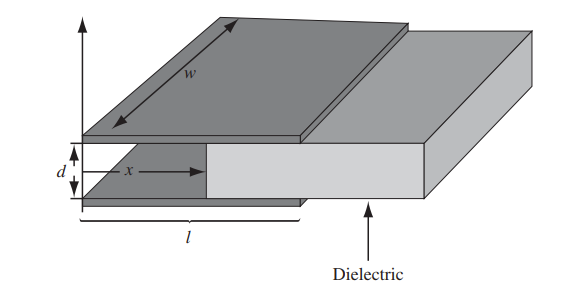
\includegraphics[width=10cm]{Electrodynamics/images/fig4.30.PNG}
\end{center}

\begin{proof}
    First, note that we need to change our model of the electric field of a parallel-plate capacitor. So far, we have assumed that the field is uniform inside, and 0 outside. If this were really true, there should be no force on the dielectric at all. However, in reality, there exists a \vocab{fringing field} around the edges which can be usually ignored, but in this case is responsible for the entire effect.
    
    \begin{center}
    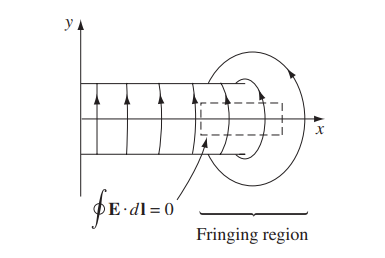
\includegraphics[width=8cm]{Electrodynamics/images/fig4.31.PNG}
    \end{center}
    
    Actually calculating fringing fields is notoriously difficult. However, we can avoid this entirely, using the following method, which analyzes the \textit{energy} involved.
    
    Let $W$ be the energy of the system; this depends on the amount of overlap between the dielectric and the capacitor. If I pull out the dielectric by an infinitesimal distance $dx$, then the energy is changed by an amount equal to the work done:
    \[dW=F_{\text{me}}\cdot dx,\]
    where $F_{\text{me}}$ is the amount of force I do to counteract the electrical force of attraction.
    
    Therefore,
    \[F=-\frac{dW}{dx}.\]
    The energy stored in the capacitor is equal to
    \[W=\frac{1}{2}CV^2,\]
    and the capacitance is
    \[C=\frac{\varepsilon_0 w}{d}(\varepsilon_r\ell-\chi_e x).\]
    If we hold the total charge on the plates constant $(Q=CV)$, then we need to use the equation (so we don't need to consider potential as a function of $x$)
    \[W=\frac{1}{2}\frac{Q^2}{C}.\]
    Then,
    \[F=-\frac{dW}{dx}=\frac{1}{2}\frac{Q^2}{C^2}\cdot\frac{dC}{dx}.\]
    However,
    \[\frac{dC}{dx}=-\frac{\varepsilon_0\chi_ew}{d},\]
    so
    \[\boxed{F=-\frac{\varepsilon_0\chi_ew}{2d}V^2}.\]
    
    We also could have chosen to instead consider what happens if we kept the capacitor at a constant potential, for example by connecting it to a battery. However, in this case, the battery also does \textit{work} as the dielectric moves, so
    \[dW=F_{\text{me}}\cdot dx+VdQ.\]
    Hence,
    \[F=-\frac{dW}{dx}+V\frac{dQ}{dx}=-\frac{1}{2}V^2\frac{dC}{dx}+V^2\frac{dC}{dx}=\frac{1}{2}V^2\frac{dC}{dx},\]
    which matches the above. Note that we had to use the equation $W=\frac{1}{2}CV^2$ instead since the potential was held constant (and we don't want to consider charge as a function of $x$).
\end{proof}

\begin{remark}
Of course, the force on the dielectric shouldn't depend on whether we hold $Q$ or $V$ constant; after all, it is solely dependent on the distribution of free and bound charges \textit{at this given moment}; we are simply displacing it by a $dx$ to see how the energy changes. Either way of solving this problem is valid, but the constant potential method is a bit trickier since we need to deal with the work from the battery.
\end{remark}

We determined the force without knowing anything about the fringing fields themselves!! 

